%%%%%%%%%%%%%%%%%%%%%%%%%%%%%%%%%%%%%%%%%%%%%%%%%%%%%
%% LaTeX2e Template by Stephen Iota (iota@usc.edu) %%
%%%%%%%%%%%%%%%%%%%%%%%%%%%%%%%%%%%%%%%%%%%%%%%%%%%%%
\documentclass{article}
\usepackage{geometry}
\usepackage[utf8]{inputenc}
%%%%%%%%%%%%%%%%%%%%%%%%%%%%%%%%%%%%%%%%%%%%%%%%%%%%%
%% LaTeX2e Template by Stephen Iota (iota@usc.edu) %%
%%%%%%%%%%%%%%%%%%%%%%%%%%%%%%%%%%%%%%%%%%%%%%%%%%%%%
\usepackage[utf8]{inputenc}
\usepackage{amsmath, amssymb, amsthm}
\usepackage{physics}
%\usepackage{algorithm}
%\usepackage[noend]{algorithmic}
\usepackage{mathtools}  % for boxed answers in align environments
%\usepackage{cancel}
\usepackage{graphicx}
\usepackage[shortlabels]{enumitem}  % change labels in enum/item envs, [noitem[list]sep]
%\usepackage[labelfont=bf,font=small]{caption}
\usepackage[dvipsnames]{xcolor}
%\usepackage[big]{titlesec}  % [small,medium,big]
%\usepackage{fancyhdr}
%\usepackage[noadjust]{cite}
%\usepackage{tikz}
\usepackage[colorlinks=true,
            citecolor=NavyBlue!90!black,
            linkcolor=green!50!black,
            urlcolor=green!50!black,
            hypertexnames=false]{hyperref}

%%%%%%%%%%%%%%%%%%%%%%%
%%%% MISC COMMANDS %%%%
%%%%%%%%%%%%%%%%%%%%%%%
\graphicspath{{./figures/}} % Setting the graphics path
\newcommand{\email}[1]{\texttt{\href{mailto:#1}{#1}}}
\newcommand{\pref}[1]{[\ref{#1}]}

%%%%%%%%%%%%%%%%%%%%
%%% FRONT MATTER %%%
%%%%%%%%%%%%%%%%%%%%
\def\makemytitle{
	\begin{center}
        {\LARGE \textsc{\nclass}: \npset}%\textbf{\npset}}
    \end{center}
    \bigbreak
    \begin{center}
        \nauthor        \\
        \email{\nemail} \\
		\nthanks        \\
        \ndate
    \end{center}
}

%%%%%%%%%%%%%%%%%%%%%%%%%%%%%%%%
%% My commands & environments %%
%%%%%%%%%%%%%%%%%%%%%%%%%%%%%%%%
%\numberwithin{equation}{section}
\theoremstyle{plain}
\newtheorem{problem}{Problem}
%\numberwithin{problem}{Problem}
\theoremstyle{definition}
%\swapnumbers % `2.1 Solution' instead of `Solution 2.1'
\newtheorem*{solution}{Solution}
%\numberwithin{solution}{solution}
\newtheorem{question}{Problem}
\renewcommand\qedsymbol{$\blacksquare$}

%%%%%%%%%%
%% MISC %%
%%%%%%%%%%
\newcommand{\nextproblem}[0]{\bigbreak}


%%%%%%%%%%%%%%%%%%%%%%%
%%%% MATH COMMANDS %%%%
%%%%%%%%%%%%%%%%%%%%%%%
\newcommand{\transpose}[1]{\ensuremath{#1^T}}
\newcommand{\colvec}[1]{\ensuremath{\begin{pmatrix} #1 \end{pmatrix}}}
\newcommand{\eye}[0]{\ensuremath{\mathbb{I}}}
\newcommand{\R}[0]{\ensuremath{\mathbb{R}}}
\newcommand{\union}[0]{\cup}
\newcommand{\intersect}[0]{\cap}
\newcommand{\set}[1]{\ensuremath{\{#1\}}}
\newcommand{\compl}[1]{\ensuremath{#1^{c}}}
\newcommand{\factorial}[1]{\ensuremath{#1!}}

\DeclareMathOperator{\Cov}{Cov}


\usepackage{caption}
\usepackage{subcaption}

%%%%%%%%%%%%%
%%% Begin %%%
%%%%%%%%%%%%%
\begin{document}

    \begin{center}
        {\LARGE \textsc{cs545 Robotics HW3:} \textbf{Inverse Kinematics}}
    \end{center}

    \bigbreak

    \begin{center}
        Stephen Iota%\footnote{SID: \texttt{6862013543}}
        \\
        \email{iota@usc.edu}
        \\
        \texttt{SID:} \texttt{6862013543}
        \\
        \today
    \end{center}

    \bigbreak

    \begin{problem}
        ~
        \begin{enumerate}
            \item[(a)] $\vb{q} = [0.,0.,0.],\ \vb{L} = [1.,1.,1.] \ \rightarrow \ fk(\vb{q}, \vb{L}) = [3., 0., 0.]$
            \item[(b)] $\vb{q} = [0.3,0.4,0.8],\ \vb{L} = [0.8,0.5,1.] \ \rightarrow \ fk(\vb{q}, \vb{L}) = [1.9215064, 1.14848143, 0.        ]$
            \item[(c)] $\vb{q} = [1.,0.,0.],\ \vb{L} = [3.,1.,1.] \ \rightarrow \ fk(\vb{q}, \vb{L}) = [3.62090692, 2.52441295, 0.        ]$
        \end{enumerate}
    \end{problem}

    \begin{problem}
        See figure \ref{fig:ik-a}.
    \end{problem}

    \begin{figure}[p]
        \centering
        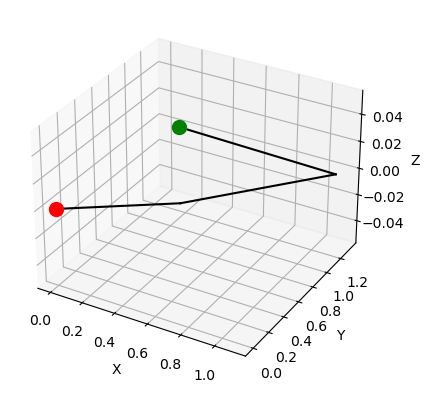
\includegraphics[width=0.5\linewidth]{ik-a_solution.png}
        \caption{Solution state computed through inverse kinematics. The base of the robot is denoted by \textcolor{red}{red}, and the goal end-effector position in \textcolor{ForestGreen}{green}. The solution state results in the robot arm touching the \phantom{ForestGreen}{green} goal state.}
        \label{fig:ik-a}
    \end{figure}

    \begin{problem}
        Implemented \texttt{line\_sphere\_intersection} in \textbf{collision.py}.
    \end{problem}

    \begin{problem}
        See figure \ref{fig:ik-b}.
    \end{problem}

    \begin{figure}[p]
        \centering
        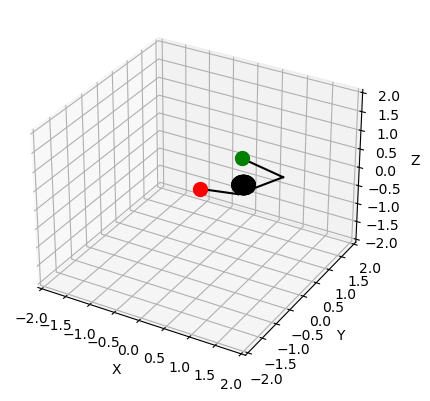
\includegraphics[width=0.45\linewidth]{ik-b_solution.png}
        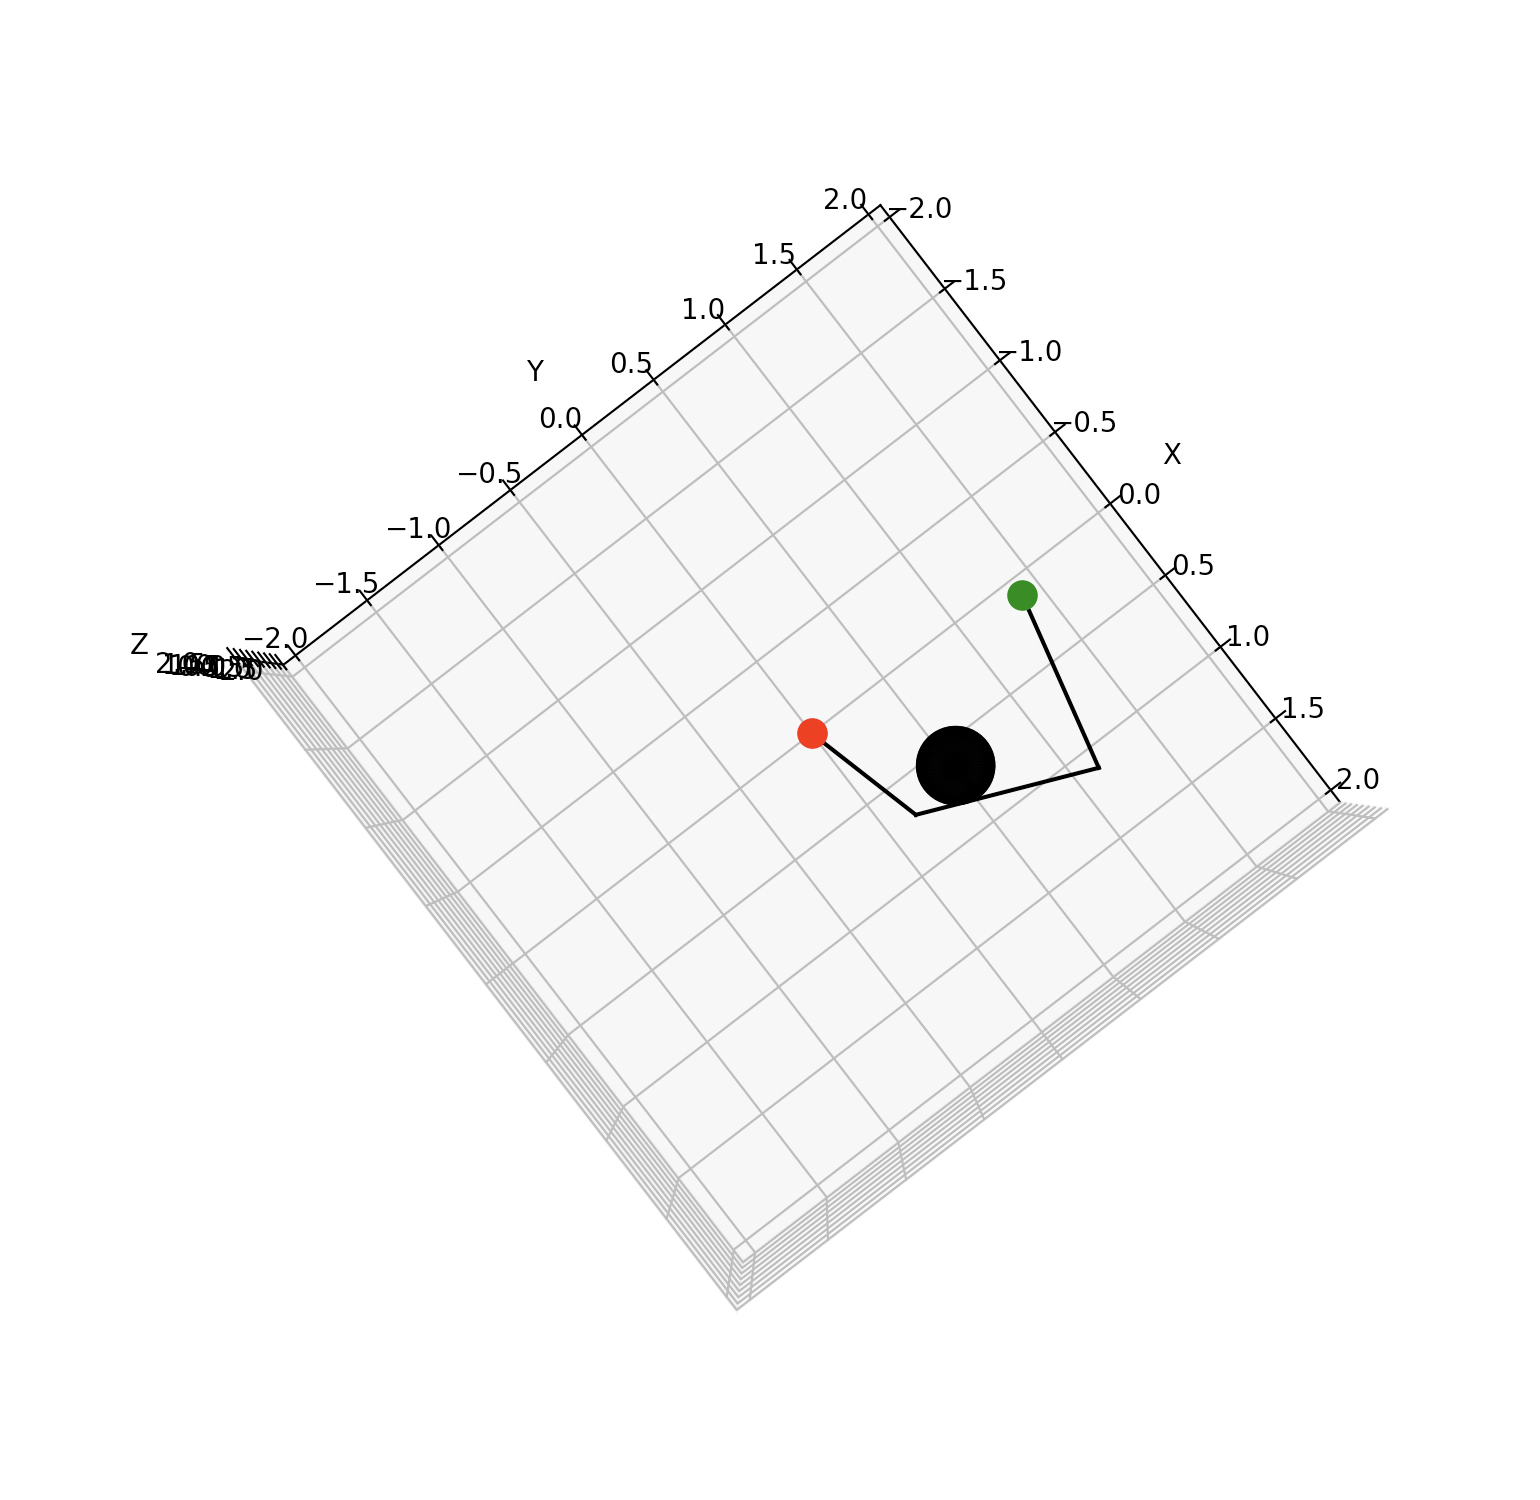
\includegraphics[width=0.45\linewidth]{ik-b2.png}
        \caption{Solution state with an obstacle (black blob), using the collision detection algorithm. In the solution state, the robot's arms reach around the obstacle to reach the goal position. The robot's second arm rests along the outside of the obstacle, as seen in the view from the top.}
        \label{fig:ik-b}
    \end{figure}

    \begin{problem}
        For larger values of $r$, solutions may not exist. If the obstacle is too big to reach around, the robot is unable to reach its end effector to the goal state. However, this can be mitigated by choosing smarter values of initial posiiton. Keeping in mind the robot joint bounds, for some starting states the robot does not need to reach around and can take a shorted path.
        For more discussion, see figure \ref{fig:5}.
    \end{problem}

    \begin{figure}
        \centering
        \includegraphics[width=0.45\linewidth]{5a.png}
        \includegraphics[width=0.45\linewidth]{5b.png}
        \includegraphics[width=0.45\linewidth]{5c.png}
        \includegraphics[width=0.45\linewidth]{5d.png}
        \caption{Top two images show different (larger) $r$ values. In these cases, there is no solution as the robot's arms are not long enough to reach around the obstacle. Bottom two figures correspond to different starting states. Noteably in the bottomleft image, due to the initial state, the robot's arms are limited by their bounds and can only overshoot the goal position.}
        \label{fig:5}
    \end{figure}

\end{document}